% We want the conclusion at the part level in the table of content but look like a chapter
% -> we shift the toclevel of everything
\makeatletter
\def\toclevel@chapter{-1}
\def\toclevel@section{0}
\def\toclevel@subsection{1}
\makeatother

% we also want the numbering to start back at A
\renewcommand{\thesection}{\Roman{section}}
\setcounter{section}{0}
%it is going to mess hyperref links because it will have the same name as previous sections -> we change it
\renewcommand*{\theHsection}{CL.\the\value{section}}
% same for figures
\renewcommand{\thefigure}{\Roman{section}.\arabic{figure}}
\setcounter{figure}{0}


\chapternonumtoc{Conclusions et Perspectives}

Nous avons étudié le comportement des deux types de moment angulaire dans la génération d'harmonique d'ordre élevé. Nous avons pu observer sa conservation, ce qui soutient la représentation de la GHOE comme un processus paramétrique. Cela permet également de transférer ces propriétés au rayonnement harmonique, c'est-à-dire à des impulsions ultra-brèves de très courte longueur d'onde. Dans ce chapitre de conclusion, nous récapitulons ces résultats et présentons les développements envisagés à partir de ces sources de lumière uniques. Nous discuterons successivement des deux composantes du moment angulaire de la lumière.

\section{Perspectives d'utilisation de rayonnement XUV portant du moment angulaire orbital}
Dans la partie \ref{CH:OAM_HHG}, nous avons d'abord discuté de la génération d'harmoniques d'ordre élevé à partir d'un faisceau de Laguerre-Gauss. Cette expérience s'ajoute à deux précédentes \mycite{ZurchNP2012,GariepyPRL2014} et étend l'étude du transfert de MAO à une gamme de paramètre bien plus large. Le moment angulaire orbital porté par le rayonnement harmonique a été caractérisé en utilisant les propriétés de divergences des faisceaux de Laguerre-Gauss, qui permet d'obtenir la loi de transfert $\ell_q=q\times\ell_1$ attendue théoriquement \mycite{HernandezPRL2013}. Contrairement aux études précédentes, qui utilisent une méthode de caractérisation directe, notre raisonnement se base uniquement sur une observation du profil d'intensité harmonique en champ lointain. Il s'appuie sur des calculs analytiques et numériques (chapitre \ref{sec:OAM_analysis}) et sur le fait que dans un processus non-linéaire, les maxima du champ émis au foyer coïncident avec ceux du champ de génération, qui est lui bien caractérisé. Cette approche indirecte est applicable quelque soit la longueur d'onde générée, ce qui nous a permis d'étudier les cas où le laser de génération porte $\ell_1=1$, $2$ ou $3$ unités de MAO. La plus haute valeur de MAO harmonique est obtenue pour $\ell_1=3$, où $\ell_{19} = 57$. Nous avons également pu étendre l'étude à des longueurs d'ondes très courtes, jusqu'à $\lambda_{41} = 19.5$ nm, en utilisant le néon comme gaz de génération.

\subsection{Génération de moment angulaire orbital arbitraire}
Ces résultats nous amènent à envisager des applications utilisant ce rayonnement aux propriétés particulière. Dans un premier temps, il serait toutefois souhaitable de disposer d'un rayonnement XUV portant de faibles valeurs de MAO. Le schéma direct présenté ici n'est pas très flexible puisque gouverné par la loi $\ell_q=q\times\ell_1$. Pour répondre à ce problème, nous avons implémenté un schéma à deux faisceaux non-colinéaires, initialement proposé par \mycite{GariepyPRL2014}. On y utilise un faisceau à 800 nm Gaussien qui croise un faisceau à 400 nm portant $\ell_1 = 1$ dans la zone d'interaction avec le jet de gaz. Ce dispositif est très similaire à celui présenté à la partie \ref{sec:calib} et se comprend dans une image photonique : l'harmonique d'ordre $q$ peut être générée par l'absorption de $q$ photons rouges, mais également de $q-4n$ photons rouges et $2n$ photons bleu. Le faisceau bleu étant non-colinéaire, la contribution du chemin $(q-4n,2n)$ sera décalée en champ lointain à mesure que $n$ augmente. De plus, le faisceau bleu portant $\ell_1=1$, la conservation du MAO impose que la contribution du chemin $(q-4n,2n)$ porte un MAO égal à $2n$. Ainsi, on peut générer à une longueur d'onde quelconque des faisceaux portant des valeurs très faibles de MAO.

Cette expérience a été réalisé à l'université de Nova Gorica, en collaboration avec le groupe de Prof. G. De Ninno. Nous présentons des résultats préliminaires sur la figure \ref{fig:gauthier}, où on observe le spectre harmonique en champ lointain. 

\begin{figure}[!ht]
\centering
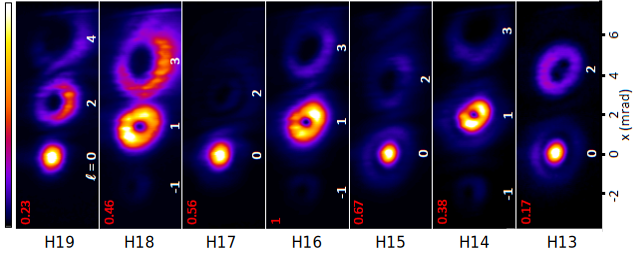
\includegraphics[width=0.8\columnwidth]{Figures/Conclusion/gauthier.pdf}%
\caption{Intensité en champ lointain obtenue à partir du schéma à deux couleurs non-colinéaires. Chaque mode est repéré par le nombre de photons bleus absorbés, c'est-à-dire par leur moment angulaire orbital.}
\label{fig:gauthier}
\end{figure}
Pour chaque harmonique, on observe de nombreux ordres de diffractions portant des valeurs de MAO différentes. Ces valeurs ont été confirmées par une mesure de front d'onde à l'aide d'un capteur de Hartmann, capable de résoudre la phase hélicoïdale pour ces faibles valeurs de $\ell$.

\subsection{Des impulsions attosecondes couplées spatio-temporellement : les light springs}
Dans un second temps, nous avons présenté une caractérisation complète du train d'impulsion attoseconde généré à partir d'un faisceau de Laguerre-Gauss. Pour ce faire, nous avons utilisé la technique RABBIT, qui permet de mesurer la phase relative entre chaque harmonique constituant le train d'impulsions. Ces mesures ont mis en évidence un problème intéressant : dans la technique RABBIT, le signal mesuré est intégré sur la totalité du volume d'interaction. Si on utilise une impulsion attoseconde portant du MAO et une impulsion d'habillage Gaussienne, la phase entre les deux faisceaux varie entre 0 et $2\pi$ dans le volume et la somme cohérente de ces contributions donne un résultat nul : les pics satellites de la trace RABBIT n'oscilleront pas. Nous avons donc utilisé une impulsion d'habillage portant le même MAO que celle de génération, de sorte à avoir un accord parfait entre les deux faisceaux au sein de la zone d'interaction. Il s'agit à notre connaissance de la première mesure de phase spectrale pour un faisceau non-Gaussien.

\subsubsection{Mesures de phase spectrale résolues spatialement}
Il est communément supposé que la phase spectrale varie peu selon les coordonnées spatiales, principalement car cette variation ne peut être résolue. En vérité, de nombreuses inhomogénéités peuvent introduire des couplages \textit{spatio-temporaux} dès l'impulsion laser de génération. On se reportera à la thèse de Gustave Pariente pour une discussion très complète sur la caractérisation de ces couplages dans le domaine infrarouge. Ils sont bien sûr transmis et amplifiés dans la GHOE, ce qui enlève une grande part de validité aux mesures intégrées spatialement. Un des axes principaux de recherche dans le domaine de la GHOE est la production d'impulsion attoseconde très énergétique, à partir de lasers de génération intenses qui interagissent sur plusieurs centimètres avec le milieu gazeuse. Il est très probable que dans ces régimes extrêmes, les couplages spatio-temporaux dans l'XUV seront un facteur limitant à l'augmentation de l'intensité sur cible.

Nos résultats suggèrent que la technique RABBIT habituelle pourrait être modifiée pour obtenir une partie de ces informations \textit{spectro-spatiales}. En effet, nous avons mis en évidence la possibilité de modifier le faisceau d'habillage pour avoir accord ou non avec le faisceau harmonique. Plutôt que d'accorder habillage et génération sur tout le volume, on pourrait restreindre de manière contrôlée la zone d'accord de sorte à mesurer la phase spectrale provenant seulement de cette partie du faisceau. Pour ce faire, il est plus simple d'utiliser l'intensité que la phase : si on utilise un faisceau d'habillage plus petit spatialement, seule la zone où les intensités des deux faisceaux sont nulles contribuera à la trace RABBIT. 

Nous avons réalisé des expériences préliminaires pour tester ce principe, dans le cadre d'une collaboration avec le groupe de Prof. L.F. DiMauro de la Ohio State University (Columbus OH, USA). Comme cas test, on cherche à caractériser un mode de Laguerre-Gauss XUV, pour lequel la phase varie linéairement avec la coordonnée azimutale. Pour le faisceau d'habillage, nous avons utilisé une lame de phase présentant une marche de $\pi$ \mycite{CamperPRA2014}. Cette lame crée au foyer deux tâches focales séparées de $\sim \SI{100}{\micro\metre}$, comme représenté sur la figure \ref{fig:spatialrabbit}. 

\begin{figure}[!ht]
\centering
\def\svgwidth{\columnwidth}
\import{Figures/Conclusion/}{spatial_rabbit.pdf_tex}
\caption{Principe d'une expérience RABBIT résolue spatialement. Le faisceau de génération (a) donne un profil de LG aux harmoniques générées. Le faisceau d'habillage (b) présente deux tâches focales, séparées d'une distance similaire au diamètre de l'anneau de génération. Ce profil peut être tourné d'un angle noté $\theta$. (c) La contribution à la mesure RABBIT est déterminée par le recouvrement entre ces deux profils d'intensité. (d) Pour chaque valeur de $\theta$, on mesure les oscillations des pics satellites dans la trace RABBIT. La phase de ces pics satellites nous donne $\phi_q(\theta)$.}
\label{fig:spatialrabbit}
\end{figure}

Si le faisceau d'habillage (\ref{fig:spatialrabbit}.b) est ajusté pour avoir une taille similaire à l'anneau du faisceau de génération (\ref{fig:spatialrabbit}.a), on peut limiter la zone contribuant à la mesure RABBIT (\ref{fig:spatialrabbit}.c). La lame de phase $0-\pi$ est montée sur une rotation motorisée, permettant de sélectionner l'angle contribuant à la trace RABBIT. Pour chaque valeur de cette angle $\theta$, on mesure les oscillations à 2$\omega$ des pics satellites. La phase de ces oscillations donne donc la phase spectrale résolue angulairement, $\phi_q(\theta)$. La figure (\ref{fig:spatialrabbit}.d) illustre le décalage entre $\theta_1$ et $\theta_1+\pi/2$ pour une phase quelconque. Pour un faisceau de Laguerre-Gauss idéal de moment $\ell_q$, on s'attend à mesurer $\phi_q(\theta) = \ell_q\theta+2\Delta t_e\omega_q$, où $\Delta t_e$ est le temps d'émission de l'atome de détection utilisé. Ces expériences n'ont pour l'instant pas été conclues, mais ce principe pourrait être généralisé à des mesures spatiales selon d'autres coordonnées.

\subsubsection{Utilisation du couplage spatio-temporel en physique ultra-rapide}
Les mesures RABBIT réalisées nous ont permis de reconstruire complètement le profil spatio-temporel du train attoseconde généré. Dans le cas de faisceaux portant du MAO, on obtient un profil d'intensité très particulier à deux spirales imbriquées. Cela met en évidence un couplage spatio-temporel très fort, où l'intensité est retardée temporellement avec la coordonnée azimutale. Nous discutons ici des possibilités d'utiliser les couplages spatio-temporels des faisceaux de LG en physique ultra-rapide.

Comme on l'a mentionné, les couplages spatio-temporels sont souvent non désirables en physique des champs forts. Toutefois, \mycite{VincentiPRL2012} ont montré qu'ils pouvaient aussi être introduits volontairement pour contrôler l'émission harmonique. Dans leur schéma, on utilise un prisme cale (\textit{wedge} en anglais) pour introduire une rotation de front d'onde au foyer au cours du temps, qui émet chaque impulsion attoseconde selon une direction angulaire donnée. \linebreak
Un faisceau de Laguerre-Gauss, de par sa phase $\ell\theta$, présente également un couplage spatio-temporel. La phase en un point donné évolue entre 0 et $\ell 2\pi$ pendant un cycle optique, on peut donc l'utiliser pour observer des phénomènes sub-cycles. Nous illustrons cette possibilité en commençant par un faisceau de Laguerre-Gauss infrarouge.

Intéressons-nous à la génération d'harmonique à deux couleurs. Dans ce schéma, des harmoniques sont générées par un faisceau à 800 nm superposé à sa deuxième harmonique, à 400 nm. Cette seconde couleur brise la centro-symétrie de la GHOE, qui était responsable de la génération d'harmoniques impaires uniquement. On obtient donc un spectre composé des harmoniques paires et impaires du laser de génération. \mycite{DudovichNP2006} ont montré que quand le champ à 400 nm est très faible, il vient simplement perturber le phénomène de GHOE habituel : au cours de l'étape de propagation du modèle à trois étapes, la trajectoire électronique est légèrement modifiée. Une analyse perturbative montre qu'en changeant le délai entre les deux couleurs, il est possible de remonter au temps d'émission électronique, ainsi qu'aux paramètres $t_i$ et $\bm{p}$ du modèle SFA \mycite{PedatzurNP2015}. L'observable mesurée ici est l'intensité harmonique en fonction du délai rouge-bleu noté $\tau$. Elle s'écrit dans le cas perturbatif et si les polarisations des champs sont parallèles :
\begin{equation}
I_q(\tau)=
\begin{cases}
I_1 + I^q_0\left|\cos(\omega_{800}\tau+\phi_q)\right|^2\text{ si $q$ impair}\\
I_2 + I^q_0\left|\sin(\omega_{800}\tau+\phi_q)\right|^2\text{ si $q$ pair}
\end{cases}
\label{eq:oren}
\end{equation}
L'information à extraire est $\phi_q$, on peut donc effectuer un scan de délai entre les deux faisceaux (figure \ref{fig:rb_mapping}.a). Une autre approche est de paramétrer ce délai spatialement de sorte à ne pas avoir à faire de scan. Prenons par exemple des faisceaux rouges et bleus portant chacun $\ell=1$. Leur phase s'écrit au point $(r,\theta)$ :
\begin{align}
\varphi_{400}(r,\theta,t) &= \omega_{400}(t + \theta/\omega_{400}),\\
\varphi_{800}(r,\theta,t) &= \omega_{800}(t + \theta/\omega_{800}).
\end{align}
Le délai les séparant s'écrit donc en tout point $\tau(r,\theta) = \theta/\omega_{800}-\theta/\omega_{400} = \theta/\omega_{400}$, ce qui est tracé en \ref{fig:rb_mapping}.b. On a donc un délai variant spatialement : le délai rouge-bleu est paramétré sur la coordonnée azimutale. On retrouvera donc l'évolution temporelle de l'intensité des harmoniques sur leur coordonnée azimutale, comme illustré sur la figure \ref{fig:rb_mapping}.c.
\begin{figure}[!ht]
\centering
\def\svgwidth{\columnwidth}
\import{Figures/Conclusion/}{rb_lg_mapping.pdf_tex}
\caption{Principe d'expériences de GHOE à deux couleurs utilisant le couplage spatio-temporel des faisceaux de LG. L'expérience habituelle est de mesurer le spectre harmonique en fonction du délai rouge-bleu (a). Si on utilise des faisceaux de LG, on a un délai variant azimutalement (b). Les harmoniques générées sont donc modulées selon $\theta$, ce qui permet de mesurer $\phi_q$ sans effectuer de scan (lignes pointillées rouges).}
\label{fig:rb_mapping}
\end{figure}
Expérimentalement, les harmoniques sont observées en champ lointain. Nous ne pouvons pas réaliser le calcul de propagation car nous ne connaissons pas la phase spatiale des harmoniques, elle aussi perturbée par le champ à 400 nm. Nous prévoyons d'effectuer des calculs SFA 4D complets pour prédire et quantifier cet effet. Dans tous les cas, l'observable $\phi_q$ se retrouvera dans le profil spatial en champ lointain. On peut donc mesurer la quantité recherchée en un seul tir laser, plutôt qu'en effectuant un scan de délai.

Dans le cas de faisceaux de Laguerre-Gauss dans l'XUV, on a la même propriété de phase paramétrée avec l'angle. De plus, si on considère non plus une harmonique donnée mais l'impulsion attoseconde entière, l'intensité a un profil de \textit{light spring}. Chaque point de l'espace $(r,\theta)$ voit donc un train d'impulsion attoseconde qui se décale temporellement de façon linéaire avec $\theta$. Cette propriété pourrait être utilisée dans une expérience d'absorption transitoire, dans laquelle on mesure habituellement l'intensité transmise par un échantillon, intégrée spatialement, au cours du temps. Avec un light spring, on pourrait plutôt résoudre spatialement l'intensité transmise, dans laquelle chaque valeur de $\theta$ correspond à une valeur de délai différente.

\subsection{Spectroscopies utilisant le moment angulaire orbital XUV}
En plus de ces couplage spatio-temporels, les faisceaux de Laguerre-Gauss possèdent un intérêt plus fondamental : les photons y portent un moment angulaire orbital bien défini. Il est très tentant de voir cette grandeur comme un paramètre supplémentaire pour contrôler et étudier l'interaction laser-matière. Par exemple, la perspective de nouvelles règles de sélection en photoionisation suggère la possibilité d'étudier des niveaux atomiques normalement interdits. Dans la partie \ref{sec:selectionrules}, nous avons montré que la réalité n'était pas si clémente : le MAO se couple préférentiellement au moment externe d'un atome. Le couplage avec le moment interne de l'atome n'apparaît qu'au second ordre. C'est également ce qui est observé dans nos mesures RABBIT : si la photoionisation était modifiée par la présence de MAO, on aurait mesuré un temps d'émission différent de celui obtenu en faisceau gaussien\footnote{En effet, le temps d'émission dépend du niveau électronique ionisé. Par exemple, \mycite{SchultzeScience2010} ont mesuré un délai de 21 as entre les électrons issus de l'orbitale 2p du néon par rapport à ceux issus de la 2s.}.

Dans notre expérience, nous disposions d'un faisceau de diamètre $\sim \SI{100}{\micro\metre}$ au foyer, à comparer avec un atome d'argon dont le diamètre est de l'ordre de l'Angström. Là est le problème principal : à l'échelle de l'atome, la phase du faisceau de LG est plate. Il n'y a qu'au centre du faisceau que la phase varie à l'échelle de l'atome, mais l'intensité y est nulle. Une transition quadripolaire dépendant du gradient du champ électrique, il est naturel qu'on ne les observe pas  dans notre cas. Pour cette raison, l'intégralité des prédictions théoriques sont jusqu'à présent limitées à des valeur d'intensité et de focalisation non réalisables en pratique. Par exemple, \mycite{PiconOE2010} prédit une modification des règles de sélection pour l'atome d'hydrogène, avec un faisceau à 27.2 eV, de waist $\SI{4.79}{\micro\metre}$ et d'intensité égale à $\SI{6.8e18}{\W\per\centi\metre\squared}$. De même, \mycite{WatzelPRA2016} proposent une mesure de délais attosecondes de nouveaux niveaux atomiques dans l'argon à partir d'un faisceau à 90 eV et d'intensité $\SI{5.6e19}{\W\per\centi\metre\squared}$.

De telles intensités dans l'XUV dépassent l'état de l'art actuel de nombreux ordres de grandeurs. S'il est certain que les intensités XUV disponibles continueront d'augmenter dans le futur, il est sûrement plus simple de chercher des systèmes plus adaptés, c'est-à-dire plus gros par rapport au faisceau harmonique. Par exemple, un atome de Rydberg a un rayon déjà bien plus important : pour le niveau n=137 de l'hydrogène, il vaut $\sim\SI{1}{\micro\metre}$. D'autres candidats sont les agrégats d'atome, ou bien des molécules de $\text{C}_{60}$, un des plus gros objets dans lequel a été observée la dualité onde-particule \mycite{ArndtNat1999}. Leur interaction avec un faisceau portant du MAO est étudié par \mycite{WatzelPRA2016}, qui observent un effet pour une intensité de $\SI{3.2e17}{\W\per\centi\metre\squared}$. L'intensité est réduite par rapport à l'argon mais pas de manière suffisante pour envisager une expérience.\linebreak
Peut-être que les cibles adaptées aux capacités expérimentales actuelles ne doivent pas être cherchées parmi les molécules, mais plutôt dans la phase condensée. Il est en effet possible de créer optiquement des excitations collectives à la surface ou dans le volume d'un solide, dont certaines pourraient être sensibles au MAO. Deux propositions intéressantes existent en ce sens : \mycite{VanVeenendaalPRL2007} prédit un dichroïsme induit par le MAO dans l'absorption au point K de métaux de transitions, tandis que \mycite{VanVeenendaalPRB2015} discute de l'interaction entre un faisceau de LG XUV et un vortex magnétique. Nous sommes en train d'évaluer la faisabilité expérimentale de ces propositions.

En conclusion, il nous semble très intéressant de continuer à développer le contrôle de faisceaux harmoniques portant du moment angulaire orbital. Les utilisations les plus immédiates nous paraissent être celles utilisant les propriétés macroscopiques de ces faisceaux. Nous avons mentionné l'utilisation de la structure spatio-temporelle des modes de LG et des impulsions attosecondes générées, qui survit dans le cas d'impulsions attosecondes isolées \mycite{HernandezPRL2013}. Il serait également assez direct d'utiliser les faisceaux de LG XUV en imagerie. En effet, ils sont déjà utilisés dans le domaine visible pour la microscopie \mycite{FurhapterOL2005} et commencent à être étudiés pour l'imagerie par diffraction cohérente \mycite{wangOE2009}. La résolution de ces deux techniques est grandement améliorée par l'utilisation de rayonnement XUV; nos résultats permettent donc d'envisager la combinaison avantageuse de faibles longueurs d'ondes et de modes de LG. \linebreak
Quant aux applications d'impulsions attosecondes portant du MAO en spectroscopie, il est probablement trop tôt pour prédire la marche à suivre. L'étude théorique de l'interaction doit continuer à se développer en se dirigeant vers des conditions plus réalistes expérimentalement, tandis que la production expérimentale de faisceaux intenses et fortement focalisés doit être optimisée dans l'XUV. Mentionnons pour terminer une autre voie de recherche ouverte par de récentes propositions \mycite{RibiPRL2014,HemsingPRL2011,HemsingPRL2012}. Elles visent à contrôler le moment angulaire orbital de lasers à électron libre, qui fournissent un rayonnement XUV très intense. Nous avons eu la chance de participer aux premiers essais d'implémentation sur FERMI (Trieste, Italie) et tenons à remercier Prof. G. De Ninno et D. Gauthier pour cette opportunité.

\section{Conclusion et perspectives sur les mesures de dichroïsme circulaire de photoélectron}